Una \textbf{criptocartera} es una herramienta que se utiliza para almacenar, 
enviar y recibir criptomonedas. Es similar a una billetera física, pero en 
lugar de contener billetes y monedas, una criptocartera contiene claves 
privadas y públicas que permiten acceder y administrar las criptomonedas.\\
\hfill \break
Cada criptomoneda tiene su propia criptocartera, y hay varios tipos de 
criptocarteras disponibles, incluyendo carteras de hardware, software y en 
línea. Las \textbf{carteras de hardware} (Figura \ref*{fig:ledger}) son dispositivos físicos que se conectan a 
un ordenador y se utilizan para almacenar las claves privadas de manera segura. 
Las \textbf{carteras de software} se descargan en un ordenador o dispositivo 
móvil y se utilizan para almacenar las claves privadas en un archivo cifrado. 
Las \textbf{carteras en línea}(Figura \ref*{fig:coinbase}) se almacenan en la nube y se pueden acceder 
desde cualquier dispositivo con una conexión a internet.
\begin{figure}[htb!]
    \caption{Criptocartera Hardware}
    \centering
    \label{fig:ledger}
    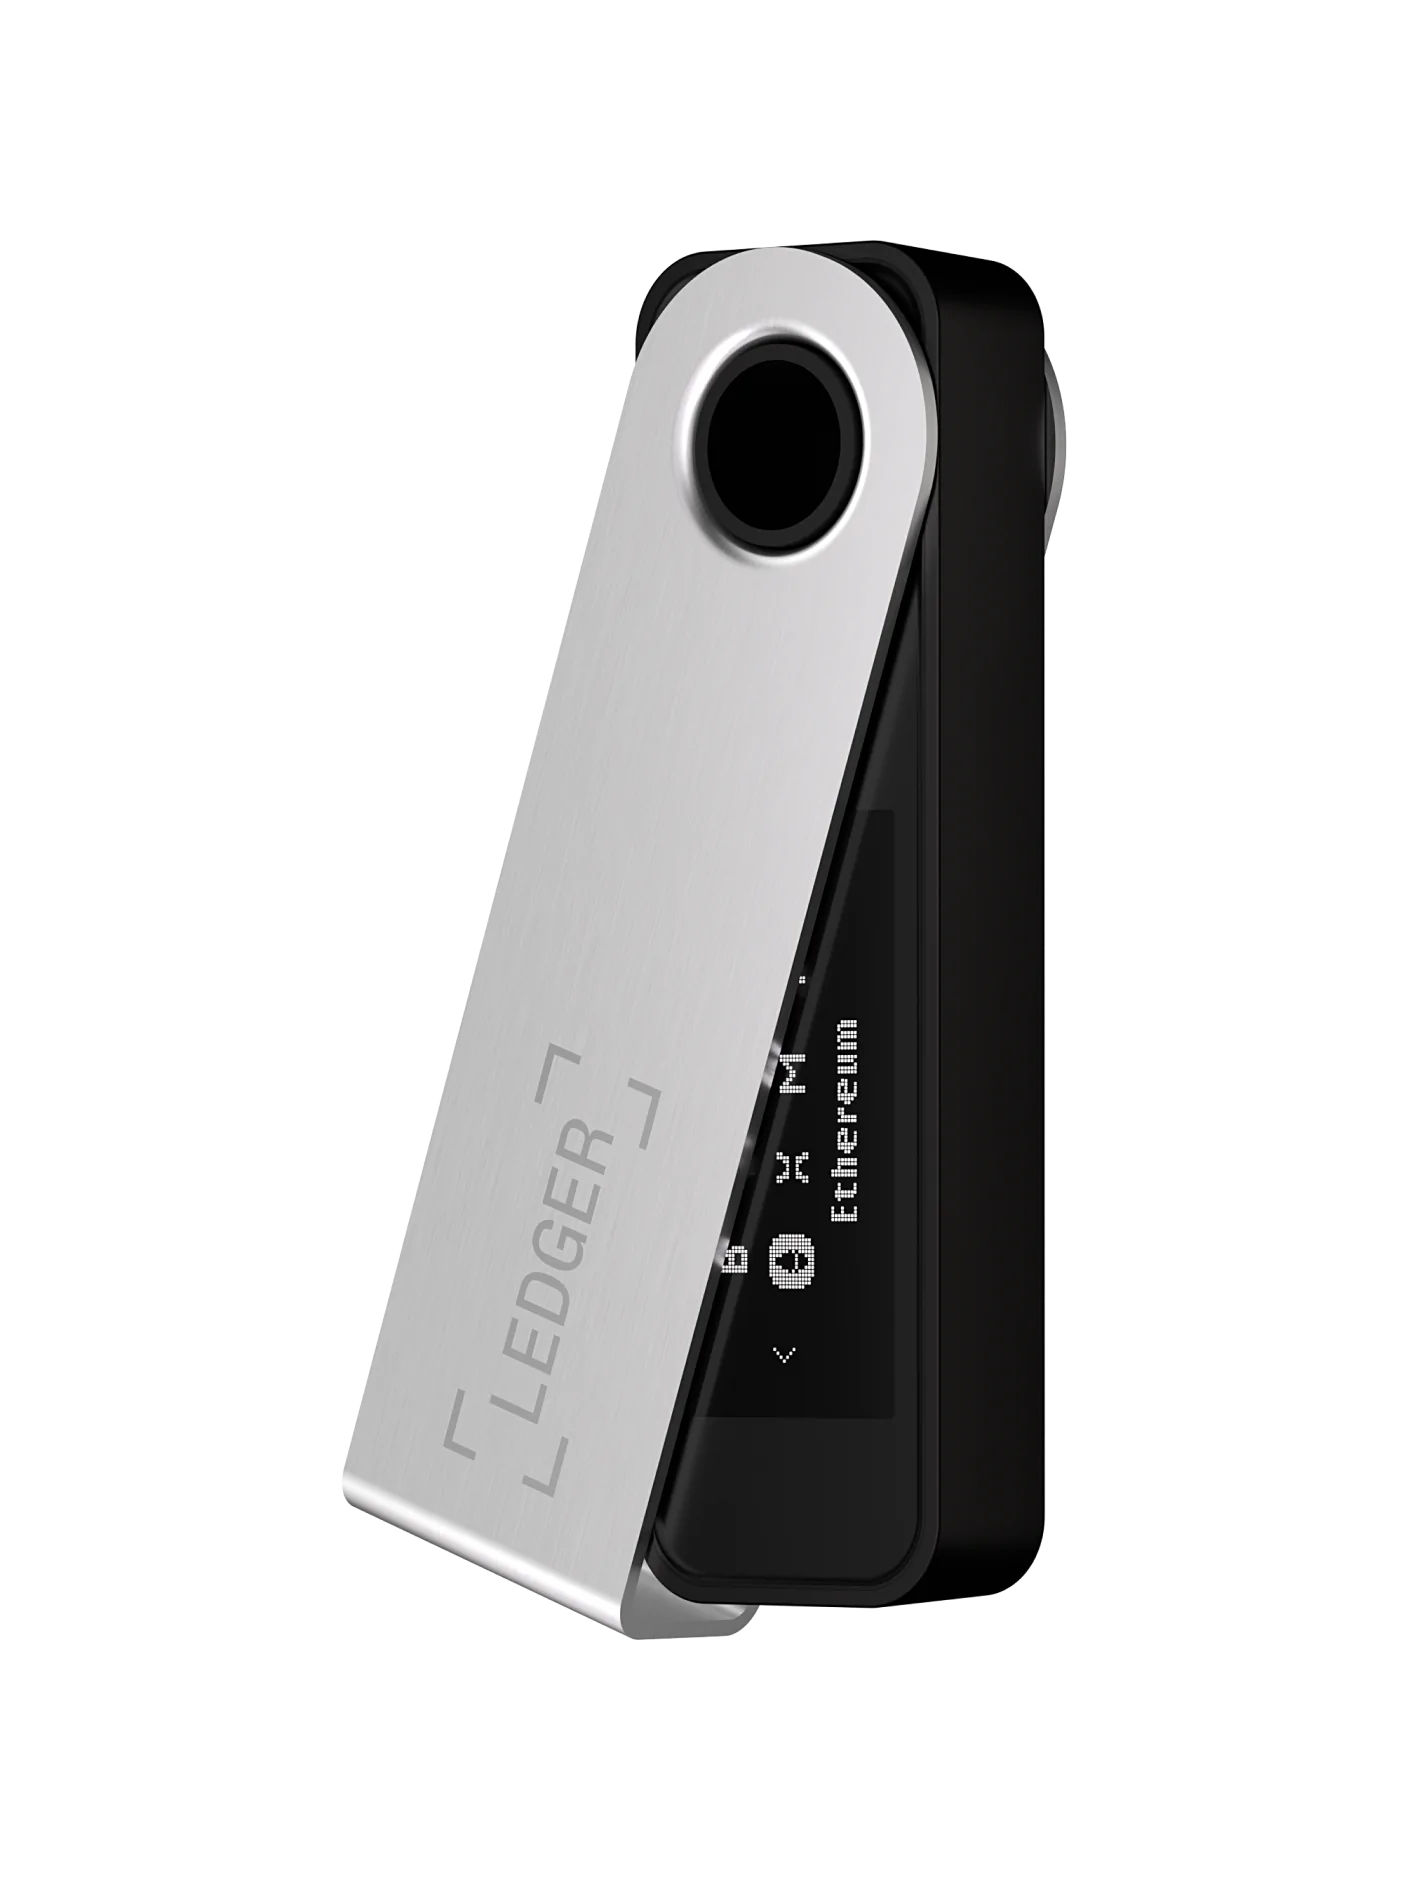
\includegraphics[scale=0.15]{./Ilustraciones/ledger-hardware.png}\\
    \textbf{Fuente:} Página oficial de Ledger [\url{https://shop.ledger.com/products/ledger-nano-s-plus}]
\end{figure}
\hfill \break
\begin{figure}[htb!]
    \caption{Criptocartera Online}
    \label{fig:coinbase}
    \centering
    
\includegraphics[scale=1]{./Ilustraciones/coinbase-logo.png}\\
    \textbf{Fuente:} Logo oficial de Coinbase  [https://www.coinbase.com/es/]
\end{figure}
Las criptocarteras son importantes porque las criptomonedas no se almacenan en 
un lugar centralizado, como un banco, sino que se almacenan en la blockchain de 
la criptomoneda. Por lo tanto, es necesario utilizar una criptocartera para 
acceder y administrar las criptomonedas.\\
\hfill \break
Las criptocarteras también permiten \textbf{enviar y recibir criptomonedas}
de forma segura. Para enviar criptomonedas, se necesita la dirección pública 
de la criptocartera del destinatario. Para recibir criptomonedas, se proporciona 
la dirección pública de la criptocartera al remitente.\\
\hfill \break
En resumen, una criptocartera es una herramienta utilizada para almacenar, 
enviar y recibir criptomonedas. Hay varios tipos de criptocarteras disponibles, 
incluyendo carteras de hardware, software y en línea. Las criptocarteras son 
importantes porque permiten acceder y administrar las criptomonedas, que se 
almacenan en la blockchain de la criptomoneda.